\newpage

\textbf{Research Plan and Methodology}\\

We describe six major tasks to be completed over two years. The project time schedule for each task is shown in Figure 1. 
%This proposed study will have two main goals, with
%sub-tasks corresponding to the six objectives specified in Part II 1(b).
%The project will be completed over two years as shown in the project time schedule
%in Figure 1.

%\begin{figure}
%	\centering
%	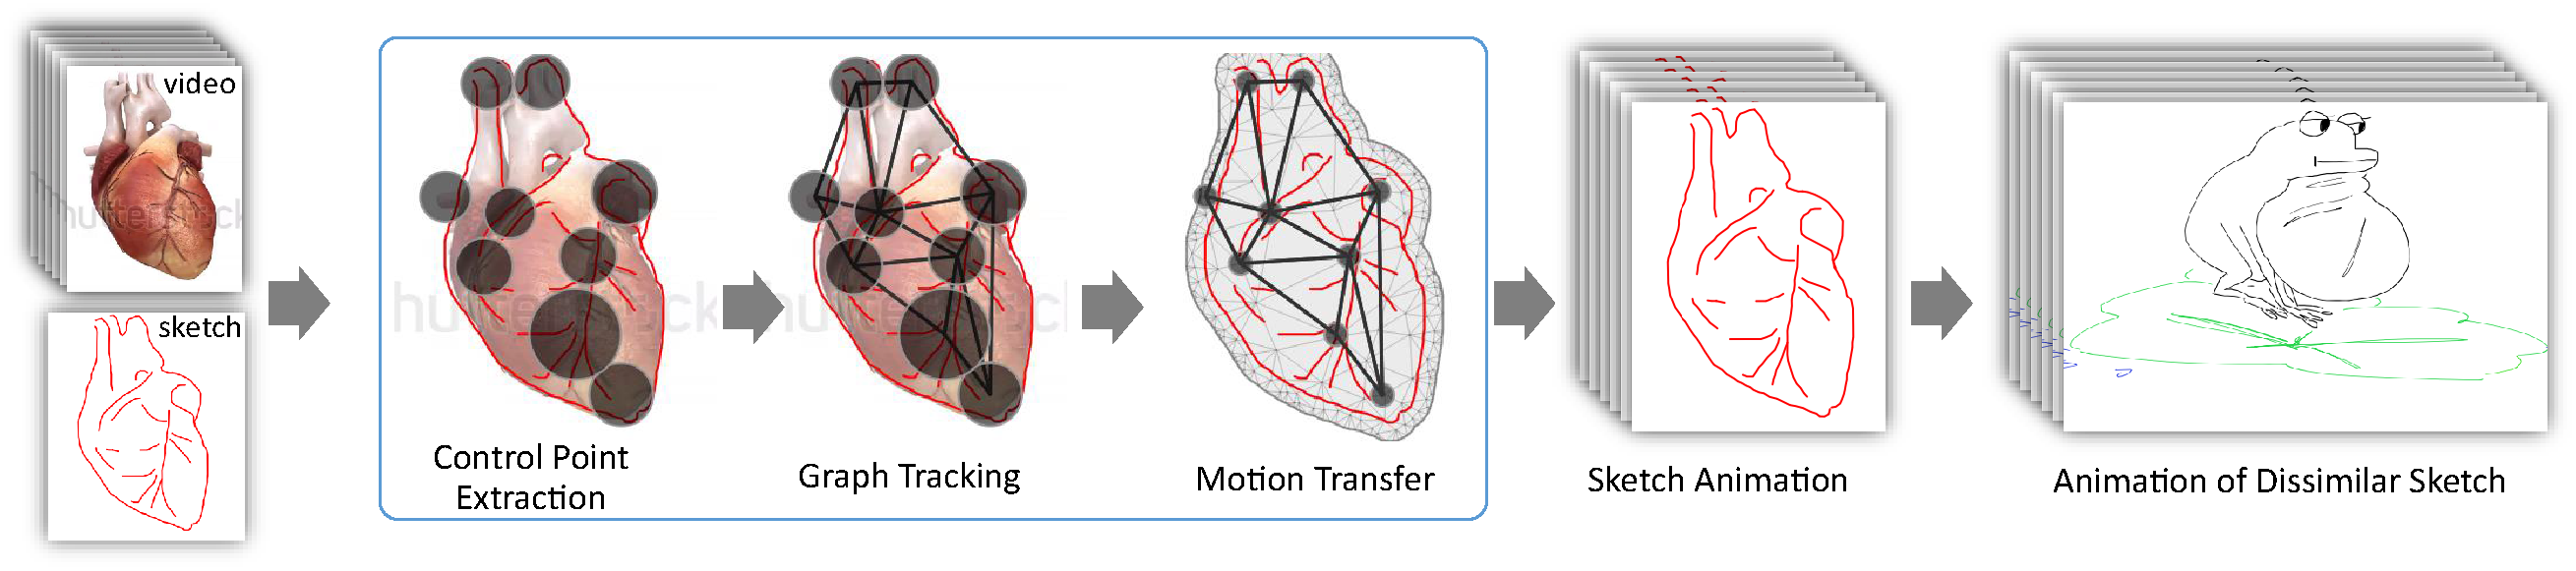
\includegraphics[width=0.85\linewidth]{images/overview}
%	\caption{}
%	\label{fig:overview}
%\end{figure}
%
%\begin{figure}
%	\centering
%	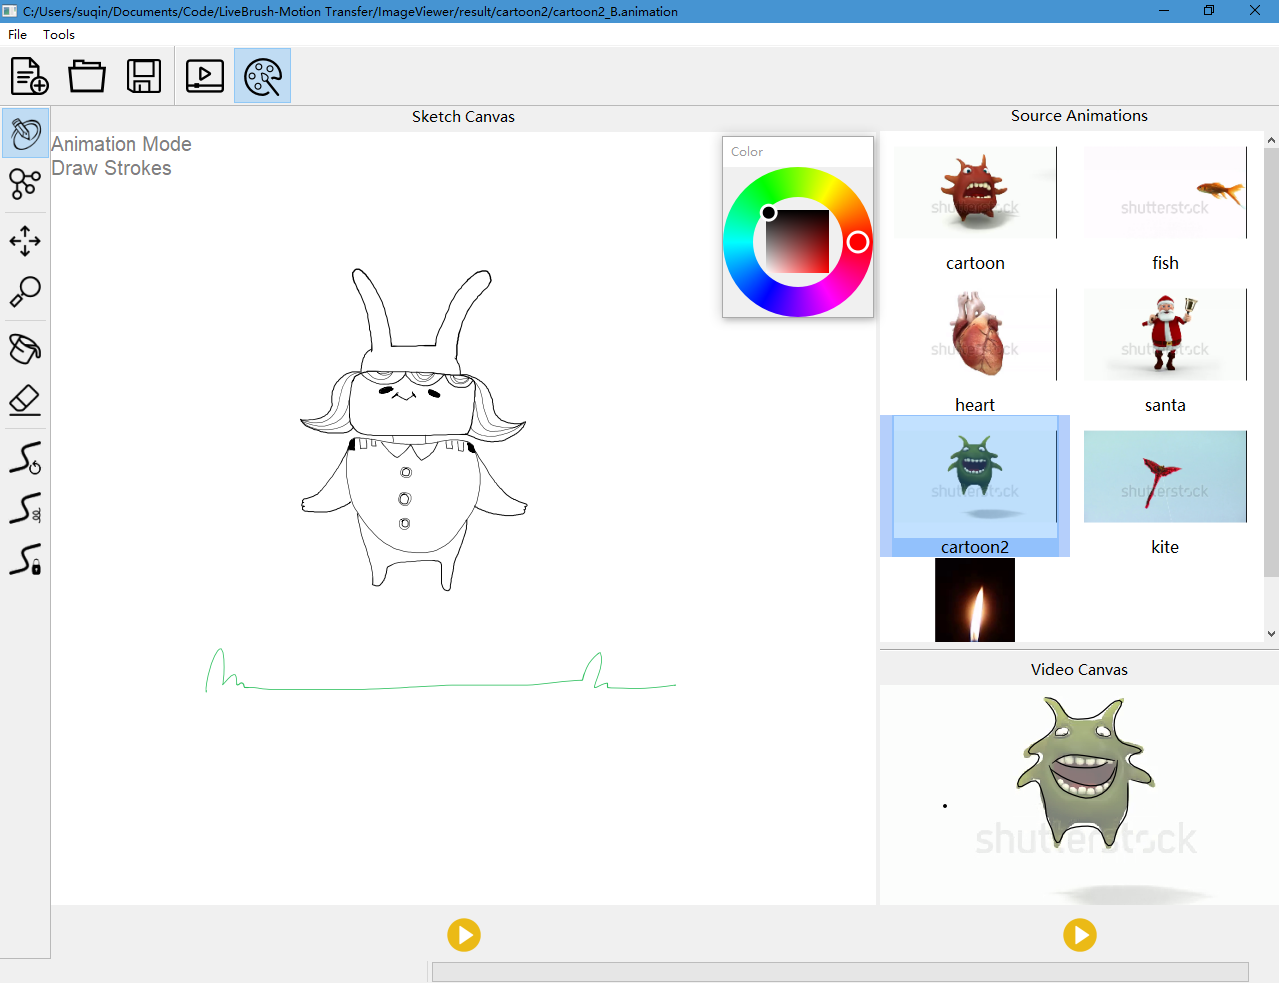
\includegraphics[width=0.85\linewidth]{images/ui}
%	\caption{}
%	\label{fig:ui}
%\end{figure}

\textbf{Task A: Interface Design}

Our system Live Sketch aims at providing novice users with an easy way to animate their drawings by an existing video. The input is a sketch and a video.
User creates a sketch by free-hand sketching and the system animates the drawing using the motion in the video automatically or with few user interactions.

The user interface ((Figure 2)) of Live Sketch, includes a tool bar, a video window, a sketch window and a playback controller. 
The tool bar lists all the tools for animation creation. 
The Video window and sketch window show the video frame and the corresponding sketch animation frame at a selected time position. 
The playback controller contains buttons for controlling the playback of the video and animation.
Users may create their drawings by free-hand sketching on the sketch window, or sketching over an image on the video window, aided by an image tracking tool~\cite{EZSketching:2014}. 
After an animation is generated, the user can select one frame of the animation for preview by moving the slider or browsing the frame list in the playback controller area.

Our system will generate the animation in three steps (Figure 3): feature points extraction and alignment, motion extraction from the video and video-to-sketch motion transfer.
\ca{The alignment step extracts good feature points from both video and sketch and compute their correspondence. Then the motion step tracks the feature points using a structure graph. The structure graph could be used for detection and position prediction of drifting points. A stroke-preserving deformation method is applied to transfer the motion to the sketch. Then the final animation is generated.}

\textbf{Task B: Feature Extraction and Alignment}

Finding the correspondence between video and sketch is a challenging problem, since the former is a bunch of meaningless pixels while the latter is graphics vector and more abstract. Our goal is to extract the feature points that are good to track the video, which also respect user's interest.

We will first extract features to track from the first video frame by scale irrelevant corner detection method~\cite{grauman:2011}.
However, some of the extracted good tracking features may have no corresponding part in the sketch, i.e., the features may not be of user's interest (gray circles in Figure 4a). In addition, the sketch and the video frame may not be well aligned (see the two examples in Figure 2 and Figure 4a,b).
Therefore, we need to filter out these feature outliers and find the correspondence between these remaining good features and the sketch.

To solve this problem, we use the same feature detection method to extract the features for the sketch image (Figure 4b). Then the optimal bipartite matching could be obtained by a non-rigid ICP point set matching method~\cite{Chui2003114}.
\ca{The matchings with large matching energy are removed from the results. The feature points without any matching are also removed. Therefore, the remaining feature points and matching results satisfies both user's interest in sketch while tracking for video.}

%$ \mathbf{P} = \{P_i | P_i = (\mathbf{x}_i, r_i)\} $ 

Sometimes the user may need to delete some extracted features to eliminate unwanted parts' animation, or add more features to include more animation details. 
Furthermore,  the structure dissimilarity between sketch and the video may be too large to extract good feature correspondence (see Figure 4c\&d).
Therefore, our user interface also allows user to manually add or remove feature points or edit their positions, and edit their flexible correspondences.
\ca{Note that even though the aided manual operations may take some time, feature extraction and alignment is only set up for only one frame and do not require any animation experience. The following two steps are efficient and fully automatic, which is the main time-consuming part in traditional keyframe-based methods. }


%\begin{figure}
%	\centering
%	\includegraphics[width=0.85\linewidth]{images/alignment}
%	\caption{Two examples}
%	\label{fig:alignment}
%\end{figure}


\textbf{Task C: Motion Extraction}


The goal of this step is to extract a robust motion trajectory for each extracted feature point of the video. However, since the final animation is very sensitive to the motion consistency of the adjacent points, we need to extract structure-preserving motion of the feature points.

We propose a structure detection and correction two-step method. During the tracking, our method first detects the drifting points and then predicts their positions by its spatial and temporal neighborhood.

The structure of the object is denoted by a structure graph over the tracking points.
The graph is constructed based on the sketch, since the sketch delivers more structure information of user's interest. 
\ca{Denote the structure graph as $ \mathcal{G} = (\mathcal{V}, \mathcal{E}) $, where $ \mathcal{V} $ is the extracted tracking features of the video. The $ \mathcal{E} $ is constructed by connecting the points in $ \mathcal{V} $ using Delaunay triangulation method. However, some edges may need to be removed, such as the 0th and 6th point in Figure 4b. To filter out these wrong edges, we compute the sketch mask for the sketch image using active contour method. Then, we remove the edges that partially locates outside of the sketch mask and all the remaining edges form the edge set $ \mathcal{E} $. }
%If two points are connected by the sketch lines or the inter-sketch parts of the path is small, they would be connected in the structure graph. 

Our structure preserving tracking method aims to solve an energy optimization problem, which contains two energy terms:
appearance energy $ E_t $, which measures the appearance difference. %  is computed for each tracking feature point using existing tracking methods such as Struck~\cite{6126251}
and structure energy $ E_s $, which measures the structure deformation errors relative to its initial structure.

To solve this optimization problem, we propose the following method. 
It first extracts a candidate set (the circles in Figure 6c,d\&e) for each extracted video feature point. Denote the candidate set of the $ i $th point as $ \mathbf{C}_i  = \{C_{ij}\}, j = 1, 2, \ldots, n_i $  with appearance energy in ascending order, where the $ j $th candidate $ C_{ij} = (\mathbf{x}_{ij}, r_{ij}) $ contains its position $ \mathbf{x}_{ij} $ and size $ r_{ij} $.
The appearance energy $ E_t $ is computed by using one state of art object tracking methods such as Struck~\cite{6126251}.

Since choosing the best candidate for each feature as the tracking result may bring in the structure distortion, we propose a detection and correction two-step method. It first detects which feature point has the largest structure energy in its the local graph, i.e. the sub-graph consisting of the point and its neighbors. Then the candidate whose structure energy is minimal and lower than a threshold $ \eta $ is chosen. If no such candidate exists, the point will be flagged as drifting and will be predicted later. Repeat this step until all the feature points have chosen the best candidate or been flagged as drifted. 
Denote the candidate combination as $ \mathbf{K} $ as $ E_s(C_{ij}|\mathbf{K}) $, where $ \mathbf{K} = (x_{1j_1}, x_{2j_2},\ldots, x_{nj_n}) $ represents the chosen candidate of each feature point.
Then the local structure energy for the $ j $th candidate $ C_{ij} $ of $ i $th feature point given the candidate combination $ \mathbf{K} $ could be computed by 

\begin{align}\label{eq:structure_energy}
E_s(C_{ij}|\mathbf{K}) = \sum_{(i, k) \in \mathcal{E}} \|(\mathbf{x}_{ij} -  \mathbf{x}_{kj_k}) - (\mathbf{x}^1_{i} -  \mathbf{x}^1_{k}) \|^2_2,
\end{align}
where $ \mathbf{x}^1_i $ represents the initial position at the first frame, which is initialized in the feature extraction step. The energy measures the edge-length difference relative to the initial position.

%Because tracking each feature independently may lead to undesired structure distortion, we preserved several candidates for each point from the tracking samples of small appearance energy.  So this could be formulated as a energy minimization problem over all candidate combinations in $ \mathcal{K} = \{\mathbf{K} | \mathbf{K} = (C_{1j_1}, C_{2j_2},\ldots, C_{nj_n})\} $
%
%\begin{align}\label{eq:motion_min}
%\mathbf{K}^* = \arg\min_{\mathbf{K} \in \mathcal{K}} \sum_{i} E(C_{ij_i}|\mathbf{K})
%= {\arg}\min_{\mathbf{K} \in \mathcal{K}} \sum_{i} E_t(C_{ij_i}|\mathbf{K}) + \alpha E_s(C_{ij_i}|\mathbf{K})
%\end{align}
%
%, where $ E_s = \sum_{(i, j) \in \mathcal{E}} \Delta d$ is measured by the edge length and angle difference regarding to initial object position.

%However, 1) it requires searching exponentially many configurations; 2) some candidates may break the structure even if they may have small appearance energy. Therefore, we will propose a method based on graph matching that could avoid the two problems(Algorithm~\ref{alg:motion_extraction}).

The algorithm is shown in Algorithm~\ref{alg:motion_extraction}. The tracking positions of drifted points can be predicted in the motion transfer step, which will be discussed later. 

\begin{algorithm}
	\caption{Motion Extraction}\label{euclid}
	\label{alg:motion_extraction}
	
	\begin{algorithmic}[1]
		\Require Video $ V $, Feature points $ \mathbf{P}^1 = \{P^1_i | P^1_i = (\mathbf{x}^1_i, r^1_i)\} $ at the first frame.
		
		\Ensure Structure preserving tracking result $ \mathbf{P}^t = \{P^t_i | P^t_i = (\mathbf{x}^t_i, r^t_i)\} $ for each frame.
		
		\State Construct the structure graph $ \mathcal{G} = (\mathcal{V}, \mathcal{E}) $.
		
		\For {$ t = 2 : m $}
		\LongState{Extract the candidate set for each feature point: $ \mathbf{C}_i  = \{C_{ij}\} $ where $ C_{ij} =
			(\mathbf{x}_{ij}, r_{ij}), j = 1, 2, \ldots, n_i$}
		
		%\State Initialization: $ \mathbf{P}^t \gets (C_{11}, C_{21}, \ldots, c_{n1}) $
		
		\LongState {Find the best candidate configuration $ \mathbf{K}^* = (C^*_1,\ldots,C^*_n) $ by finding the best candidate for each feature point to minimize the structure energy (Eq.~\ref{eq:structure_energy}). The drifting feature points $  \mathbf{S} = \{i | E(C^*_i|\mathbf{K}^*) > \eta \} $ are also detected. $ \forall i \notin \mathbf{S}, P^t_i \gets C^*_i. $}
		\LongState {Predict bad matching point's position $ \{ P^t_i | i \in \mathbf{S}\} $ by spatial neighbors in motion transfer step.} 
		\EndFor
		
		\State Refine the drifting point's position $ \{ P^t_i | i \in \mathbf{S}\} $ its global motion trajectory.
		
		\State \Return $ \{\mathbf{P}^t\} $.
		%		\While {true}
		%		\State $ i^* \gets \max_i E_t(C^*_i) + \alpha E_s(C^*-C^*_i) $
		%		\State $ j^* \gets \min_j E_t(c_{i^*j}) + \alpha E_s(C^*-C^*_{i^*} + c_{i^*j}) $
		%		
		%		\EndWhile
		%		
		%		\State $\textit{stringlen} \gets \text{length of }\textit{string}$
		%		\State $i \gets \textit{patlen}$
		%		\If {$i > \textit{stringlen}$} \Return false
		%		\EndIf
		%		\State $j \gets \textit{patlen}$
		%		\If {$\textit{string}(i) = \textit{path}(j)$}
		%		\State $j \gets j-1$.
		%		\State $i \gets i-1$.
		%		\State \textbf{goto} \emph{loop}.
		%		\State \textbf{close};
		%		\EndIf
		%		\State $i \gets i+\max(\textit{delta}_1(\textit{string}(i)),\textit{delta}_2(j))$.
		%		\State \textbf{goto} \emph{top}.
		%		\State \Return $ C $
		
	\end{algorithmic}
\end{algorithm}

%Existing related work that try to resolve this problem, such as single or object tracking using geometric model~\cite{Martinez20083682,Artner20111969,6243144,6934993,zhang2013structure}, which could tolerant some drifting problems or matching errors. However, these methods usually used a global optimization for all parts/objects, which may lead to either a global drifting problem when using strong structure constraint, or structure distortion at some parts/object because of using strong appearance trackers. 
Our method is different with structure-preserving previous single/multiple object tracking methods. Previous structure-preserving single object tracking methods~\cite{Martinez:2008,Artner:2011,Cehovin:2013,Cai:2014} usually weak local features of sampled patches to track one single window. Therefore, the accuracy of tracking each patch is unstable. They do not require the detection and prediction of the drifting points. The structures used in existing multiple object tracking methods\cite{Zhang:2013} is different with ours. They are usually more flexible and do not have so strong global relationship. Furthermore, they are usually one step tracking method and do not correct their positions when drifting problem happens.

%methods~\cite{Martinez:2008,Artner:2011,Cehovin:2013,Cai:2014,Zhang:2013}, including the structure preserved multi-object tracking methods, our method is a detection and correction two-step method. It insures to avoid sketch distortion after the motion is transfered. 


\textbf{Task D: Motion Transfer}

Motion transfer aims to apply the extracted motion (Task C) to the sketch respecting the extracted correspondence (Task B). We will derive a variant of as-rigid-as possible(ARAP) mesh deformation method~\cite{Igarashi:2005}.
To animate the sketch by deformation, we will first generate a mesh by triangulating the sketch mask region obtained in Task B.
%To generate the mesh for sketch deformation, we triangulate the contour that is obtained using active contour method for the sketch image.
Therefore, the sketch could be animated by moving sketch feature points.
However, ARAP mesh deformation itself can not preserve the stroke shape because it only keeps the rigidibility of the mesh triangles (see Figure 4a). 

Therefore, we will propose a stroke-preserving ARAP method to preserve the stroke shape during the mesh deformation. The main idea of our method is that the original mesh will try to indirectly deform the sketch through new constructed intermediate triangles. Therefore, the original mesh deformation becomes a soft force to the sketch rather than the hard force using interpolation method.

%Denote the feature positions of the $ t $th and $ (t + 1) $th frame as $ \mathbf{p}^t = \{p^t_{i}\} $ and $ \mathbf{p}^{t+1} = \{p^{t + 1}_{i}\} $.
In order to achieve such effect, we modify the original mesh (gray in Figure 4a) $ \mathcal{M}_0 = (\mathcal{V}_0, \mathcal{T}_0) $ by adding all the sampled stroke points $ \mathcal{V}_s $ and constructing two triangle sets $ \mathcal{T}_s $ and $ \mathcal{T}_l $.
\textit{Sketch triangle} set $\mathcal{T}_s $ is constructed by connecting every three successive points on each stroke (purple triangles in Figure 4a).
\textit{Link triangle} set $\mathcal{T}_l $ is constructed by connecting each sketch point with its three vertices of the triangle containing it.
%(cyan triangles in Figure 4a).

%\begin{figure}[t]
%	\centering
%	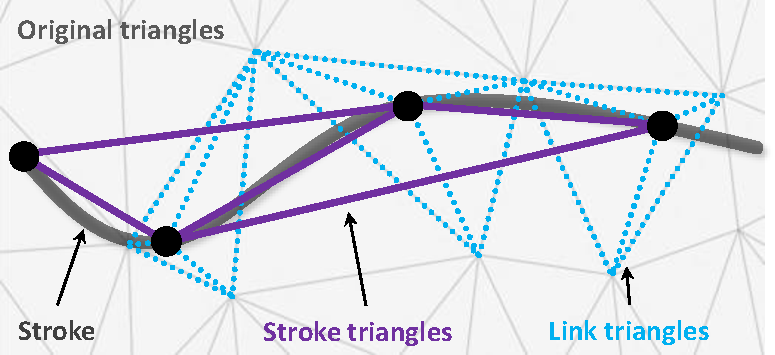
\includegraphics[width = 0.95\linewidth]{images/mesh}
%	\caption{Reconstructed mesh for stroke-preserving ARAP deformation.}
%	
%	\label{fig:mesh}	
%\end{figure}

Then, our ARAP mesh deformation is applied to the modified mesh $ \mathcal{M} = (\mathcal{V}_0 \cup \mathcal{V}_s, \mathcal{E}_0 \cup \mathcal{T}_s \cup \mathcal{T}_l) $ by the following energy minimization formulation:
\begin{align}
\min_\mathcal{M} E_0 + E_{link} + \beta E_{sketch},
\end{align}
where $ E_0 $ is deformation energy of the original mesh $ \mathcal{M}_0 $ relative to the original mesh position, $ E_{1ink} $ and $ E_{sketch} $ represents the deformation energy of the new constructed triangle sets $\mathcal{T}_s $ and $\mathcal{T}_l $. Minimizing $ E_{sketch} $ keeps the shape of the strokes and  $ E_{link} $ transfers the deformation of the original mesh to the strokes. The weight of $ E_{link} $ is set to 1 so that it could be as rigid as the original mesh, the weight of the stroke triangles, $ \beta $, to be large ($ > $ 1) so that the shape of the strokes is preserved. 

Figure 5 shows the results of our stroke-preserving ARAP deformation method and existing ARAP deformation method. Observe that our method is able to preserve the shape of the stroke.

\ca{\textbf{Prediction of drifting points in Task C}. Note that the drifting points are not used as the handles of the mesh deformation, because their positions is unreliable. Our method predict their positions by their spatial and temporal neighbors. First, their positions are interpolated by the post-deformed mesh. In addition, their positions may not be consistent with their temporal neighborhood, which leads to shuffling problems at these drifting frame positions. Therefore, we also smooth the trajectories of these drifting points. }

\textbf{Task E: Evaluation}

%Our system aims at providing the user with an easy way to add 3D strokes to an existing shape for communicating conceptual design ideas. Strokes drawn by a user over an existing 3D shape are generally of two types. The first type lie on an existing surface. The 3D information for such a stroke can be determined easily by projection onto the surface. The second type of strokes are drawn to specify a non-existent part of the shape, indicating how the original shape is to be modified. Determining the 3D information for this type of stroke is nontrivial. Our system focuses on providing an interface to draw sketch strokes of the second type.

We will conduct a user study to evaluate our system. The user study will consist of two parts. In User Study I, a number of participants will be invited to create two sketch animations for each example using our system and existing state of art methods. It will be designed to collect user feedback on the usability of our system and the evaluate efficiency of our system. In this experiment, the participants will be asked to create a sketch animation to a given video. We will compare the completion time and the number of operations which include sketching operations and editing operations using our tools and existing tools. After they finish their animation, they will be asked to answer a questionnaire to evaluate features of the two ways.
The sketch animation created using the two methods will then be evaluated by a different group of participants in User Study II.
We ask the participants to score each sketch animation that is created in User Study I on the aesthetics, completeness, etc. 


\textbf{Task F: Other Extensions}

Since our live brush tool aims to animate a sketch using the same motion of the object in the video, it may look as real as the video. Therefore, we propose to provide post animation stylization tools to make the animation more stylized, such as using animation filter~\cite{Wang:2006}, the 12 animation principles~\cite{Kazi:2016}, animation looping, etc.

\ca{In our system, we focus on motion transfer a single object. We will also propose a tool to create animations containing numerous objects. Therefore, we need to design and implement a new user interface that can combine the results of several animation results of our method into one scene.}

Our tool is used for creating sketch animation, it would be more popular if we could move it to touch-based devices like iPad or iPhone. This requires us to redesign the user UI and improve the efficiency to improve the user experience.

%In our system, we require only coplanar strokes be drawn in each step. This setting ensures that our system is able to generate the expected 3D sketch with only simple interaction. However, this restriction may hinder the user during drawing. The ultimate goal of allowing the user to draw strokes on arbitrary planes or surfaces in any order is too difficult. Instead, we will further investigate how to make our system more general by introducing other type of constraints besides the coplanar constraint for drawing strokes, constraining the current set of drawn curves to be on a curved surface, or to be symmetric. 
%%\ca{Similar to the current algorithm, we will borrow the geometry information to constrain the drawn curves. Specifically, 
%If the matched sharp edges are on a common curved surface that is extracted from the shape, the surface is a potential canvas. If the drawn strokes are self-symmetrical after an affine transformation, the canvases that realize this transformation might be desirable ones. When the user draws a set of strokes, it is unknown which constraint should be used. A possible solution will be to traverse all the constraints and generate all possible candidate 3D strokes which will be ranked using the same criteria described before.

%An issue to solve then would be how does the system automatically recognize what type of constraint to enforce on the drawn strokes. \ca{Possible solutions? curved surface derived from the given shape}



\newpage


%Man-made shape is the main focus of our system. It is because designing man-made shapes is more common than organic shapes. 
%For example, the user may want to modify the design of an existing furniture model, or change the appearance of a building model. When designing a 3D scene, the models in this scene are mostly man-made. In our system, we will mainly focus on the following information.

